\documentclass[12pt,a4paper]{article}
\usepackage{amsmath,amsthm,tikz}
\usepackage[euler-digits]{eulervm}
%%%%%%%%%%%%%%%%%%%%%%%%%%%%%%%%%%%%%%%%%%%%%%%%%%%%%%%%%%%%%%%%%%%%%
\newtheorem{theorem}{Theorem}
\newcommand{\iprod}[1]{\langle#1\rangle}
\newcommand{\vecp}[1]{\boldsymbol{p}}
\newcommand{\hatvecp}{\hat{\boldsymbol{p}}}
%%%%%%%%%%%%%%%%%%%%%%%%%%%%%%%%%%%%%%%%%%%%%%%%%%%%%%%%%%%%%%%%%%%%%
\title{Notes on Gauss Quadrature for General Weight Functions}
\author{Bill McLean}
\date{\today}
%%%%%%%%%%%%%%%%%%%%%%%%%%%%%%%%%%%%%%%%%%%%%%%%%%%%%%%%%%%%%%%%%%%%%
\begin{document}
\maketitle
%%%%%%%%%%%%%%%%%%%%%%%%%%%%%%%%%%%%%%%%%%%%%%%%%%%%%%%%%%%%%%%%%%%%%
\section{Three-term recurrence relation}
Given a finite positive measure~$\nu$ on the real line, we define 
an inner product and norm on the space of all (real) polynomials by
\[
\iprod{f,g}=\int f(x)g(x)\,d\nu(x)\quad\text{and}\quad
\|f\|=\sqrt{\iprod{f,f}}.
\]
Using the Gram--Schmidt procedure to orthogonalise the linearly 
independent monomials $1$, $x$, $x^2$, $x^3$, \dots, defining the 
monic polynomial~$p_j(x)$ of degree~$j$ by
\[
p_j(x)=x^j-\sum_{k=0}^{j-1}\frac{\iprod{x^j,p_k}}{\|p_k\|^2}\,p_k(x)
	\quad\text{for $j=0$, $1$, $2$, \dots.}
\]
In this way,
\begin{equation}\label{eq: orthog}
\iprod{p_j,p_k}=0\quad\text{if $j\ne k$.}
\end{equation}

\begin{theorem}\label{thm: 3 term}
The orthogonal polynomials defined above satisfy the three-term 
recurrence relation
\[
p_j(x)=(x-a_j)p_{j-1}(x)-b_j^2p_{j-2}(x)
	\quad\text{for $j=1$, $2$, $3$, \dots,}
\]
with $p_0(x)=1$ and $p_{-1}(x)=0$. The coefficients satisfy
\[
a_j=\frac{\iprod{xp_{j-1},p_{j-1}}}{\|p_{j-1}\|^2}
\quad\text{and}\quad
b_j=\frac{\|p_{j-1}\|}{\|p_{j-2}\|},
\]
except that, by convention, we put $b_1=\sqrt{\int d\nu}$.
\end{theorem}
\begin{proof}
Since $p_j(x)-xp_{j-1}(x)$ has degree at most~$j-1$, there are 
constants~$c_{jk}$ such that
\[
p_j(x)-xp_{j-1}(x)=\sum_{k=0}^{j-1}c_{jk}p_k(x).
\]
Taking the inner product of both sides with~$p_{j-1}$ and using
the orthogonality property~\eqref{eq: orthog}, we obtain
\[
-\iprod{xp_{j-1},p_{j-1}}=c_{j,j-1}\|p_{j-1}\|^2,
\]
showing that $c_{j,j-1}=-a_j$.  Also, taking the inner product of both
sides with~$p_k$ for $k\le j-3$ gives
\[
c_{jk}\|p_k\|^2=\iprod{p_j-xp_{j-1},p_k}=-\iprod{p_{j-1},xp_k}=0,
\]
so $p_j(x)=(x-a_j)p_{j-1}(x)+c_{j,j-2}p_{j-2}(x)$ and
\[
0=\iprod{p_j,p_{j-2}}=\iprod{xp_{j-1},p_{j-2}}+c_{j,j-2}\|p_{j-2}\|^2.
\]
Finally, 
\begin{align*}
\iprod{xp_{j-1},p_{j-2}}&=\iprod{p_{j-1},xp_{j-2}}
	=\iprod{p_{j-1},p_{j-1}}+\iprod{p_{j-1},xp_{j-2}-p_{j-1}}\\
	&=\|p_{j-1}\|^2+0,
\end{align*}
and therefore $c_{j,j-2}=-\|p_{j-1}\|^2/\|p_{j-2}\|^2=-b_j^2$.
\end{proof}

We denote the ortho\emph{normal} polynomials by
\[
\hat p_j(x)=\frac{p_j(x)}{\|p_j\|},
\]
and find that
\[
b_{j+1}\hat p_j(x)=(x-a_j)\hat p_{j-1}(x)-b_j\hat p_{j-2}(x),
\]
or equivalently,
\begin{equation}\label{eq: 3 term orthog}
b_j\hat p_{j-2}(x)+a_j\hat p_{j-1}(x)+b_{j+1}\hat p_j(x)=xp_j(x).
\end{equation}
Defining
\[
T_n=\begin{bmatrix}
a_1&b_2   &       &       &\\
b_2&a_2   &b_3    &       &\\
   &\ddots&\ddots &\ddots &\\
   &      &b_{n-1}&a_{n-1}&b_n\\
   &      &       &b_n    &a_n
\end{bmatrix}
\quad\text{and}\quad
\hatvecp_n(x)=\begin{bmatrix}p_0(x)\\ p_1(x)\\ \vdots\\ p_{n-1}(x)
\end{bmatrix},
\]
the equations~\eqref{eq: 3 term orthog} for $0\le j\le n-1$ are 
equivalent to
\[
T_n\hatvecp_n(x)+b_{n+1}\hat p_n(x)\boldsymbol{e}_n=x\hatvecp_n(x).
\]

\subsection{Legendre polynomials}
The Legendre polynomials have the orthogonality property
\begin{equation}\label{eq: legendre orthog}
\int_{-1}^1 P_k(x)P_l(x)\,dx=\frac{2\delta_{kl}}{2k+1}
\end{equation}
and the 3-term recurrence relation is
\begin{equation}\label{eq: legendre 3 term}
kP_k(x)=(2k-1)xP_{k-1}(x)-(k-1)P_{k-2}(x).
\end{equation}
The normalised Legendre polynomials are
\[
\hat P_k(x)=\frac{P_k(x)}{\|P_k\|}=\biggl(\frac{2k+1}{2}\biggr)^{1/2}
	P_k(x),
\]
and thus
\begin{multline*}
k\biggl(\frac{2}{2k+1}\biggr)^{1/2}\hat P_k(x)
	=(2k-1)\biggl(\frac{2}{2k-1}\biggr)^{1/2}x\hat P_{k-1}(x)\\
	-(k-1)\biggl(\frac{2}{2k-3}\biggr)^{1/2}\hat P_{k-2}(x),
\end{multline*}
or equivalently,
\[
\frac{k\hat P_k(x)}{\sqrt{2k+1}}=\sqrt{2k-1}\,x\hat P_{k-1}(x)
	-\frac{k-1}{\sqrt{2k-3}}\,\hat P_{k-2}(x).
\]
Thus, the Legendre polynomials satisfy
\[
b_{k+1}\hat P_k(x)=(x-a_k)\hat P_{k-1}(x)-b_k\hat P_{k-2}(x)
\]
where
\[
a_k=0\quad\text{and}\quad b_k=\frac{k-1}{\sqrt{(2k-1)(2k-3)}},
\]
except that $b_1=\sqrt{\int_{-1}^1\,dx}=\sqrt{2}$.



\section{The modified Chebyshev algorithm}
Following Gautschi~\cite{Gautschi1982} we consider the sequence of 
monic orthogonal polynomials $q_0$, $q_1$, $q_2$ generated by a 
positive measure $\mu$ on the real line.  Thus, $q_k$ is a monic 
polynomial of degree~$k$ and
\[
\int q_j(x)q_k(x)\,d\mu(x)=0\quad\text{for all $j\ne k$.}
\]
We write the three-term recurrence relation as
\begin{equation}\label{eq: 3 term q}
q_k(x)=(x-\alpha_k)q_{k-1}(x)-\beta_k^2 q_{k-2}(x)
	\quad\text{for $k=1$, $2$, $3$, \dots,}
\end{equation}
with
\[
q_0(x)=1\quad\text{and}\quad q_{-1}(x)=0.
\]
We adopt the usual convention that $\beta_0=\sqrt{\int d\mu}$.

Our aim is to use the modified Chebyshev algorithm to determine the 
coefficients $\alpha_k$~and $\beta_k$ for $1\le k\le n$.
This algorithm uses a second family of monic orthogonal 
polynomials, say $p_0$, $p_1$, $p_2$, \dots, having known coefficients 
$a_k$~and $b_k$ 
in the associated three-term recurrence relation
\[
p_k(x)=(x-a_k)p_{k-1}(x)-b_k^2p_{k-2}(x)
	\quad\text{for $k=1$, $2$, $3$, \dots,}
\]
with $p_0(x)=1$~and $p_{-1}(x)=0$.  Let $\nu$ denote the associated 
positive measure, so that
\[
\int p_j(x)p_k(x)\,d\nu(x)=0\quad\text{for all $j\ne k$.}
\]

\begin{figure}
\caption{The dots correspond to the $\sigma_{lk}$ computed in the 
case~$n=5$.  The parallelogram indicates the $\sigma_{lk}$ used in 
the expressions for $\alpha_5$~and $\beta_5$.}
\begin{center}
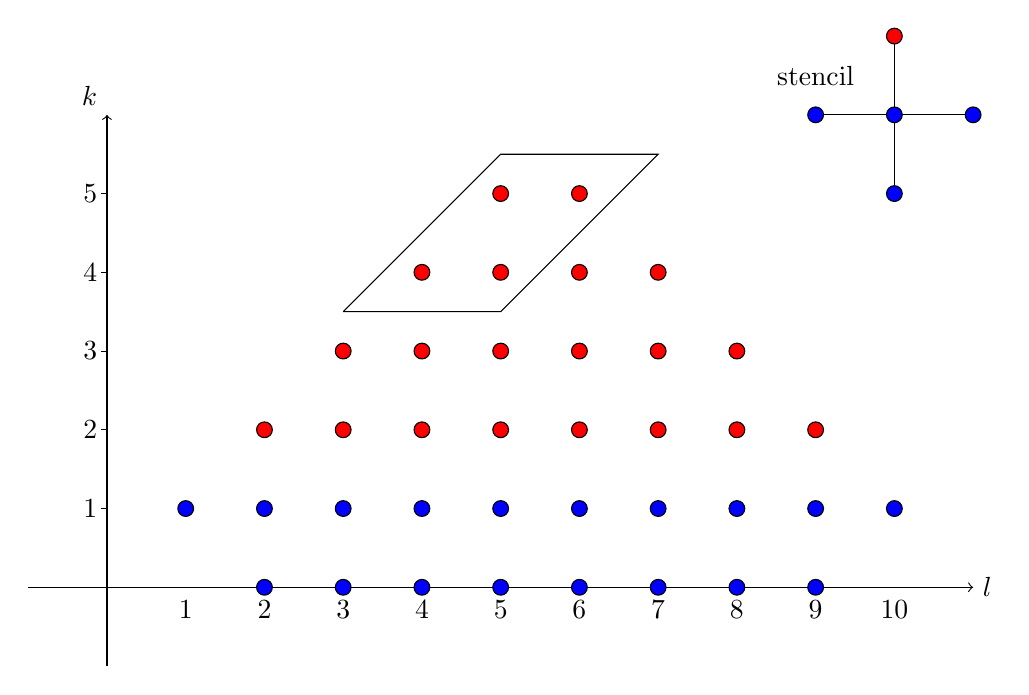
\begin{tikzpicture}[scale=1.0]
\draw[->] (0, -1) -- (0, 6);
\node[above left] at (0, 6) {$k$};
\draw[->] (-1, 0) -- (11, 0);
\node[right] at (11, 0) {$l$};
\foreach \x in {2, 3, ..., 9}
    \draw[fill=blue] (\x, 0) circle(0.10cm);
\foreach \x in {1, 2, ..., 10}
    \draw[fill=blue] (\x, 1) circle(0.10cm);
\foreach \x in {2, 3, ..., 9}
    \draw[fill=red] (\x, 2) circle(0.10cm);
\foreach \x in {3, 4, ..., 8}
    \draw[fill=red] (\x, 3) circle(0.10cm);
\foreach \x in {4, 5, 6, 7}
    \draw[fill=red] (\x, 4) circle(0.10cm);
\foreach \x in {5, 6}
    \draw[fill=red] (\x, 5) circle(0.10cm);
\foreach \y in {1, 2, 3, 4, 5}
    {
    \draw[thin] (-0.075, \y) -- (0, \y);
    \node[left] at (0.0, \y) {$\y$};
    }
\foreach \x in {1, 2, 3, ..., 9, 10}
    \node[below] at (\x, -0.04) {$\x$};
\draw[-] (10, 5) -- (10, 7);
\draw[-] (9, 6) -- (11, 6);
\draw[fill=blue] (9, 6) circle(0.10cm);
\draw[fill=blue] (10, 6) circle(0.10cm);
\draw[fill=blue] (11, 6) circle(0.10cm);
\draw[fill=blue] (10, 5) circle(0.10cm);
\draw[fill=red]  (10, 7) circle(0.10cm);
\node at (9, 6.5) {stencil};
\draw[-] (3.0, 3.5) -- (5.0, 5.5) -- (7.0, 5.5) 
      -- (5.0, 3.5) -- (3.0, 3.5);
\end{tikzpicture}
\end{center}
\end{figure}

The algorithm requires that we know the values of the integrals
\[
\mu_k=\int p_{k-1}(x)\,d\mu(x)\quad\text{for $1\le k\le 2n$,}
\]
and is summarised in the following theorem.

\begin{theorem}
The coefficients $\alpha_1$, $\alpha_2$, \dots, $\alpha_n$~and 
$\beta_0$, $\beta_1$, \dots, $\beta_{n-1}$ in the three-term 
recurrence relation~\eqref{eq: 3 term q} can be computed by putting
\[
\begin{aligned}
\sigma_{l,0}&=0&\text{for $2\le l\le 2n-1$},\\
\sigma_{l,1}&=\mu_l&\text{for $1\le l\le2n$},\\
\alpha_1&=a_1+\frac{\mu_2}{\mu_1},\\
\beta_1&=\sqrt{\mu_1},
\end{aligned} 
\]
and, for $k=1$, $2$, \dots, $n-1$ and $k\le l\le2n-k-1$, 
\[
\begin{aligned}
\sigma_{l+1,k+1}&=\sigma_{l+2,k}+(a_l-\alpha_k)\sigma_{l+1,k}
		+b_l^2\sigma_{lk}-\beta_k^2\sigma_{l+1,k-1},\\
\alpha_{k+1}&=a_{k+1}+\frac{\sigma_{k+2,k+1}}{\sigma_{k+1,k+1}}
	-\frac{\sigma_{k+1,k}}{\sigma_{kk}},\\
\beta_{k+1}&=\sqrt{\frac{\sigma_{k+1,k+1}}{\sigma_{kk}}}.
\end{aligned}
\]
\end{theorem}
\begin{proof}
It is easily verified that the integrals
\[
\sigma_{lk}=\int p_{l-1}(x)q_{k-1}(x)\,d\mu(x)
\]
satisfy the initial conditions $\sigma_{l,0}=0$~and 
$\sigma_{l,1}=\mu_l$.  In addition, $\sigma_{lk}=0$ if $k>l$. 
For $1\le k\le l$,
\begin{align*}
\sigma_{l+1,k+1}&=\int p_l(x)\bigl[
(x-\alpha_k)q_{k-1}(x)-\beta_k^2q_{k-2}(x)\bigr]\,d\mu(x)\\
	&=\int(x-a_l+a_l-\alpha_k)p_l(x)q_{k-1}(x)\,d\mu(x)
		-\beta_k^2\sigma_{l,k-2}\\
	&=\int\bigl[(x-a_l)p_l(x)-b_l^2p_{l-1}(x)\bigr]
		q_{k-1}(x)\,d\mu(x)\\
	&\qquad{}+(a_l-\alpha_k)\sigma_{l+1,k}
		+b_l^2\sigma_{lk}-\beta_k^2\sigma_{l+1,k-1}
\end{align*}
so
\[
\sigma_{l+1,k+1}=\sigma_{l+2,k}+(a_l-\alpha_k)\sigma_{l+1,k}
		+b_l^2\sigma_{lk}-\beta_k^2\sigma_{l+1,k-1}.
\]

By Theorem~\ref{thm: 3 term},
\[
\alpha_{k+1}=\int xq_k(x)^2\,d\mu(x)\bigg/\int q_k(x)^2\,d\mu(x)
\]
and
\[
\beta_{k+1}^2=\int q_k(x)^2\,d\mu(x)\bigg/\int q_{k-1}(x)^2\,d\mu(x).
\]
Since $q_k(x)-p_k(x)$ has degree at most~$k-1$, the orthogonality 
property of the $q_k$ implies that
\begin{align*}
\int q_k(x)^2\,d\mu(x)&=\int p_k(x)q_k(x)\,d\mu(x)
	+\int\bigl[q_k(x)-p_k(x)\bigr]q_k(x)\,d\mu(x)\\
	&=\sigma_{k+1,k+1}+0,
\end{align*}
so
\[
\beta_{k+1}^2=\frac{\sigma_{k+1,k+1}}{\sigma_{kk}}
	\quad\text{for $k\ge1$,}
	\qquad\text{with $\beta_1^2=\mu_1$.}
\]
Similarly,
\[
\int x q_k(x)^2\,d\mu(x)
	=\int x\bigl[q_k(x)-p_k(x)\bigr]q_k(x)\,d\mu(x)
	+\int xp_k(x)q_k(x)\,d\mu(x),
\]
with
\begin{align*}
\int x&\bigl[q_k(x)-p_k(x)\bigr]q_k(x)\,d\mu(x)
	=\int\bigl[q_k(x)-p_k(x)\bigr](x-\alpha_{k+1})q_k(x)\,d\mu(x)\\
	&\qquad\qquad\qquad\qquad\qquad\qquad{}+\alpha_{k+1}\int 
		\bigl[q_k(x)-p_k(x)\bigr]q_k(x)\,d\mu(x)\\
	&=\int\bigl[q_k(x)-p_k(x)\bigr]
	\bigl[q_{k+1}(x)+\beta_{k+1}^2 q_{k-1}(x)\bigr] 
		\,d\mu(x)+\alpha_k\times0\\
	&=-\beta_{k+1}^2\sigma_{k+1,k}
	=-\frac{\sigma_{k+1,k+1}}{\sigma_{kk}}\,\sigma_{k+1,k}
\end{align*}
and
\begin{align*}
\int xp_k(x)q_k(x)\,d\mu(x)&=\int\bigl[
	(x-a_{k+1})p_k(x)-b_{k+1}^2p_{k-1}(x)\bigr]q_k(x)\,d\mu(x)\\
	&\qquad{}+\int\bigl[
		a_{k+1}p_k(x)+b_{k+1}^2p_{k-1}(x)\bigr]q_k(x)\,d\mu(x)\\
	&=\int p_{k+1}(x)q_k(x)\,d\mu(x)
		+a_{k+1}\int p_k(x)q_k(x)\,d\mu(x)\\
	&=\sigma_{k+2,k+1}+a_{k+1}\sigma_{k+1,k+1};
\end{align*}
thus,
\[
\alpha_{k+1}=a_{k+1}+\frac{\sigma_{k+2,k+1}}{\sigma_{k+1,k+1}}
	-\frac{\sigma_{k+1,k}}{\sigma_{kk}}
	\quad\text{for $k\ge1$,}
\]
with
\[
\alpha_1=\frac{\sigma_{21}+a_1\sigma_{11}-\beta_0\sigma_{1,0}}%
{\sigma_{11}}=a_1+\frac{\sigma_{21}}{\sigma_{11}}
	=a_1+\frac{\mu_2}{\mu_1}.
\]
\end{proof}
%%%%%%%%%%%%%%%%%%%%%%%%%%%%%%%%%%%%%%%%%%%%%%%%%%%%%%%%%%%%%%%%%%%%%
\section{A log weight}
We now consider the example
\[
d\mu(x)=x^\rho\log x^{-1}\,dx\quad\text{for $0<x<1$,}
\]
with $\rho>-1$.  As our second family of orthogonal polynomials we 
use the monic shifted Legendre polynomials,
\[
p_k(x)=\frac{P_k(2x-1)}{C_k}
\quad\text{where}\quad
C_k=\binom{2k}{k};
\]
thus
\[
C_k\mu_k=\int_0^1 P_k(2x-1)x^\rho\log x^{-1}\,dx.
\]
Following \cite{Gautschi1979}, we make the substitution $y=2x-1$
and obtain
\[
C_k\mu_k=\frac{\log 2}{2^{\rho+1}}\int_{-1}^1 P_k(y)(y+1)^\rho\,dy
	-\frac{1}{2^{\rho+1}}\int_{-1}^1 
		P_k(y)(y+1)^\rho\log(y+1)\,dy
\]
It is known that
\[
\int_{-1}^1 P_k(y)(y+1)^\rho\,dy
	=\frac{2^{\rho+1}\Gamma(\rho+1)^2}%
{\Gamma(\rho+k+2)\Gamma(\rho+1-k)},
\]
and by logarithmic differentiation of this identity with respect 
to~$\rho$, we find that
\begin{multline*}
\int_{-1}^1 P_k(y)(y+1)^\rho\log(y+1)\,dy
	=\frac{2^{\rho+1}\Gamma(\rho+1)^2}%
{\Gamma(\rho+k+2)\Gamma(\rho+1-k)}\\
	\times\bigl[\log2+2\psi(\rho+1)-\psi(\rho+k+2)-\psi(\rho+1-k)
	\bigr],
\end{multline*}
where $\psi(x)=\Gamma'(x)/\Gamma(x)$ denotes the digamma function.
Thus,
\begin{multline}\label{eq: mu k}
C_k\mu_k=\frac{\Gamma(\rho+1)^2}{\Gamma(\rho+k+2)\Gamma(\rho+1-k)}\\
	\times\bigl[\psi(\rho+k+2)+\psi(\rho+1-k)-2\psi(\rho+1)\bigr].
\end{multline}
Using the reflection formulae
\[
\Gamma(1-z)\Gamma(z)=\frac{\pi}{\sin\pi z}
\quad\text{and}\quad
\psi(1-z)=\psi(z)+\pi\cot\pi z,
\]
we find that
\[
\lim_{z\to m}\frac{1}{\Gamma(-z)}=0
\quad\text{and}\quad
\lim_{z\to m}\frac{\psi(-z)}{\Gamma(-z)}=(-1)^{m+1}m!
\]
for $m\in\{0,1,2,\dots\}$.  Thus, if $\rho=r\in\{0,1,2,\dots\}$
then
\[
C_k\mu_k=(-1)^{k-r}\,\frac{(r!)^2(k-r-1)!}{(k+r+1)!}
	\quad\text{for $k\in\{r+1, r+2, r+3, \dots\}$.}
\]
Otherwise, we can use the functional identities
\[
\Gamma(z+1)=z\Gamma(z)\quad\text{and}\quad
\psi(z+1)=\psi(z)+\frac{1}{z}
\]
to simplify \eqref{eq: mu k}.  In fact,
\[
\Gamma(\rho+1)=\rho(\rho-1)\cdots(\rho+1-k)\Gamma(\rho+1-k)
\]
and
\[
\Gamma(\rho+k+2)=(\rho+k+1)(\rho+k)\cdots(\rho+2)(\rho+1)
	\Gamma(\rho+1),
\]
so
\begin{align*}
\frac{\Gamma(\rho+1)^2}{\Gamma(\rho+k+2)\Gamma(\rho+1-k)}
	&=\frac{\rho(\rho-1)\cdots(\rho+1-k)}%
{(\rho+k+1)(\rho+k)\cdots(\rho+2)(\rho+1)}\\
	&=\frac{1}{\rho+1}\prod_{j=1}^k\frac{\rho+1-j}{\rho+1+j}.
\end{align*}
Moreover,
\[
\psi(\rho+k+2)=\psi(\rho+1)+\frac{1}{\rho+1}+\frac{1}{\rho+2}
	+\cdots+\frac{1}{\rho+k+1}
\]
and
\[
\psi(\rho+1-k)=\psi(\rho+1)-\frac{1}{\rho}-\frac{1}{\rho-1}
	-\cdots-\frac{\rho-(k-1)},
\]
so
\[
\psi(\rho+k+2)+\psi(\rho+1-k)-2\psi(\rho+1)
	=\frac{1}{\rho+1}+\sum_{j=1}^k\biggl(\frac{1}{\rho+1+j}
		-\frac{1}{\rho+1-j}\biggr).
\]
Hence,
\[
C_k\mu_k=\frac{1}{\rho+1}\biggl[\frac{1}{\rho+1}
	+\sum_{j=1}^k\biggl(\frac{1}{\rho+1+j}
		-\frac{1}{\rho+1-j}\biggr)\biggr]
	\prod_{j=1}^k\frac{\rho+1-j}{\rho+1+j}.
\]

In view of \eqref{eq: legendre orthog}~and 
\eqref{eq: legendre 3 term}, the shifted monic Legendre polynomials 
satisfy
\[
\int_0^1p_k(x)p_l(x)\,dx=\frac{\delta_{kl}}{(2k+1)C_k^2}
\]
and
\begin{align*}
p_k(x)&=\frac{kP_k(2x-1)}{kC_k}
	=\frac{(2k-1)(2x-1)P_{k-1}(2x-1)-(k-1)P_{k-2}(x)}{kC_k}\\
	&=(2k-1)(2x-1)\frac{C_{k-1}}{kC_k}p_{k-1}(x)
		-\frac{k-1}{k}\,\frac{C_{k-2}}{C_k}\,p_{k-2}(x),
\end{align*}
with $p_0(x)=1$ and $p_{-1}(x)=0$.  Moreover,
\[
C_k=\frac{(2k)!}{(k!)^2}=\frac{(2k)(2k-1)}{k^2}\,C_{k-1}
	=\frac{2(2k-1)}{k}\,C_{k-1}
\]
so
\[
\frac{C_{k-1}}{C_k}=\frac{k}{2(2k-1)}
\quad\text{and}\quad
\frac{C_{k-2}}{C_k}=\frac{C_{k-2}}{C_{k-1}}\,\frac{C_{k-1}}{C_k}
	=\frac{k-1}{2(2k-3)}\,\frac{k}{2(2k-1)}.
\]
Hence, $p_k(x)=(x-a_k)p_{k-1}(x)-b_{k-1}^2p_{k-2}(x)$ where
\[
a_k=\frac{1}{2}\quad\text{and}\quad
b_k^2=\frac{k^2}{2^2(2k-1)(2k+1)},
\]
except $b_0=\sqrt{\int_0^1\,dx}=1$.








%%%%%%%%%%%%%%%%%%%%%%%%%%%%%%%%%%%%%%%%%%%%%%%%%%%%%%%%%%%%%%%%%%%%%
\bibliographystyle{plain}
\bibliography{notes_refs}
%%%%%%%%%%%%%%%%%%%%%%%%%%%%%%%%%%%%%%%%%%%%%%%%%%%%%%%%%%%%%%%%%%%%%
\end{document}
\endinput
